\documentclass[12pt]{book} 

\usepackage{amsmath}
\usepackage{graphicx}
\usepackage{import}
\usepackage{amsfonts}
\usepackage{booktabs}

\setlength{\parindent}{0em}  % sets auto indent at new paragraph to none

\newcommand{\incfig}[1]{%
    \import{./figures/}{#1.pdf_tex}
}

\title{\coursetitle\linebreak\lecturename}
\author{\\Cain Susko\\ 
           \\ \\ \\
      Queen's University 
    \\School of Computing\\} 

%=-=-=-=-=-title-=-=-=-=-=%
\newcommand{\lecturename}{Machine Representation of Programs: Data}
\newcommand{\coursetitle}{Computer Architecture}
%=-=-=-=-=-#####-=-=-=-=-=%

\begin{document}
\begin{titlepage}
        \maketitle
\end{titlepage}


\section*{Arrays}
Arrays are a way of storing data of the same type:
\[
\texttt{T A[L]}
.\] 
This is an array $A$ of data Type  $T$ and length $L$. Additional Examples are:
\begin{figure}[h]
        \centering
        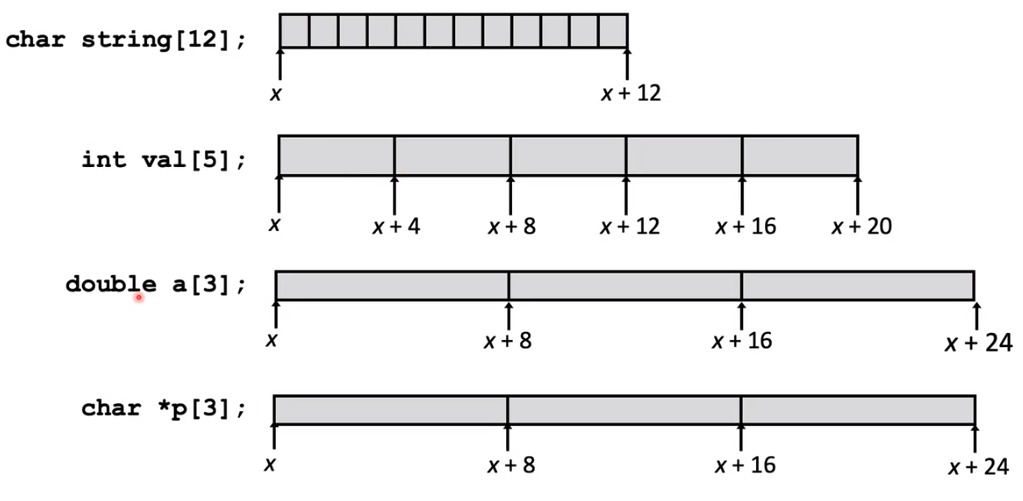
\includegraphics[scale = 0.3]{./figures/arrayEx}
\end{figure}

Arrays can be accessed using pointers like so:
\begin{figure}[h]
        \centering
        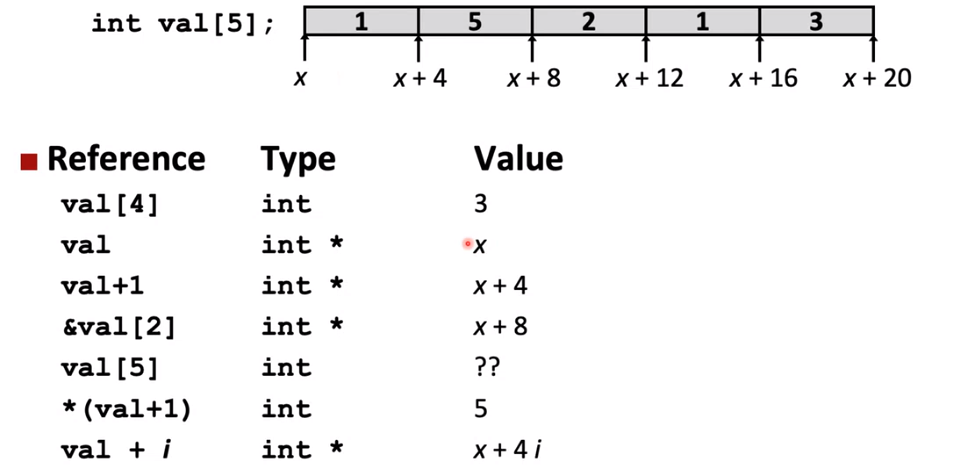
\includegraphics[scale = 0.4]{./figures/arrayPointers}
\end{figure}

Note: $val$ is equal to the pointer at the start of the array.
\pagebreak
\subsection*{1D Arrays}

A comprehensive example of an array is the following:
\begin{figure}[h]
        \centering
        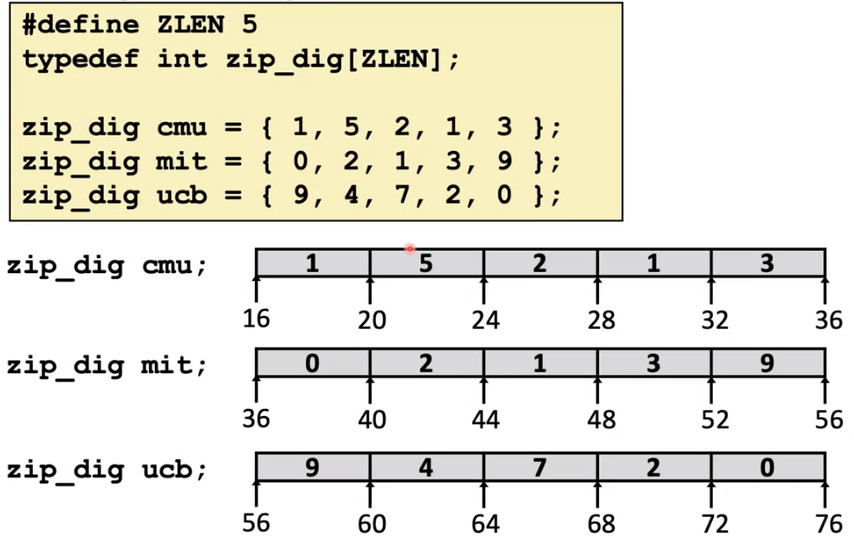
\includegraphics[scale = 0.2]{./figures/arrayEx2}
        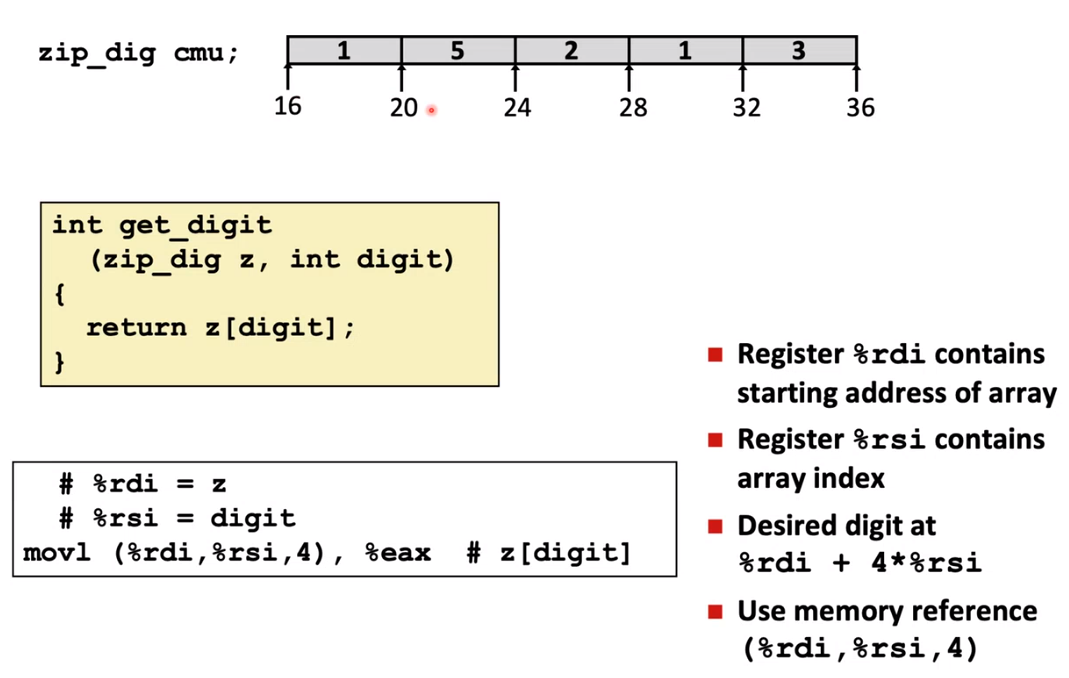
\includegraphics[scale = 0.2]{./figures/arrayEx3}
\end{figure}

Consider the example of a n Array in a loop:
\begin{figure}[h]
        \centering
        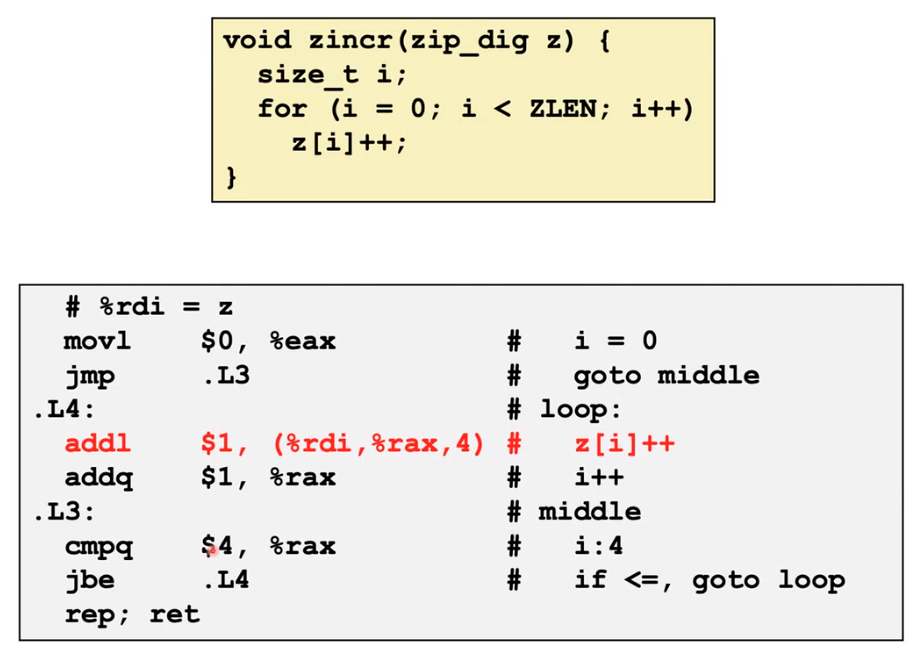
\includegraphics[scale = 0.3]{./figures/loop1}
\end{figure}
Note: this is just one of many forms of loops we covered in a previous lesson.
Additionally, note that the $ret$ instruction is used but there is no value returned 
(acceptable usage).

\subsection*{Multi-Dimensional Arrays}
the declaration of a multi-dimensional or nested array is:
\[
\texttt{T A[R][C]}
.\] 
where $A$ is an array of objects with type  $T$ as well as $R$ rows and  $C$ columns.
The size of the array can be found by doing $R\times C\times k-bytes$.
\pagebreak

The arrangement in memory or a 2D array is row majored, meaning theyre stored row by row, 
linearly in memory:
\begin{figure}[h]
        \centering
        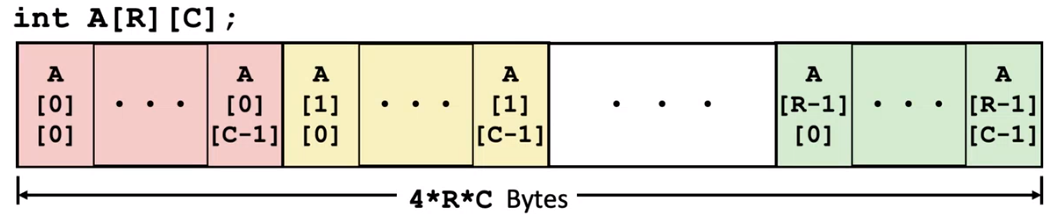
\includegraphics[scale = 0.3]{./figures/arrayStruct}
\end{figure}

Consider the following nested array example:
\begin{figure}[h]
        \centering
        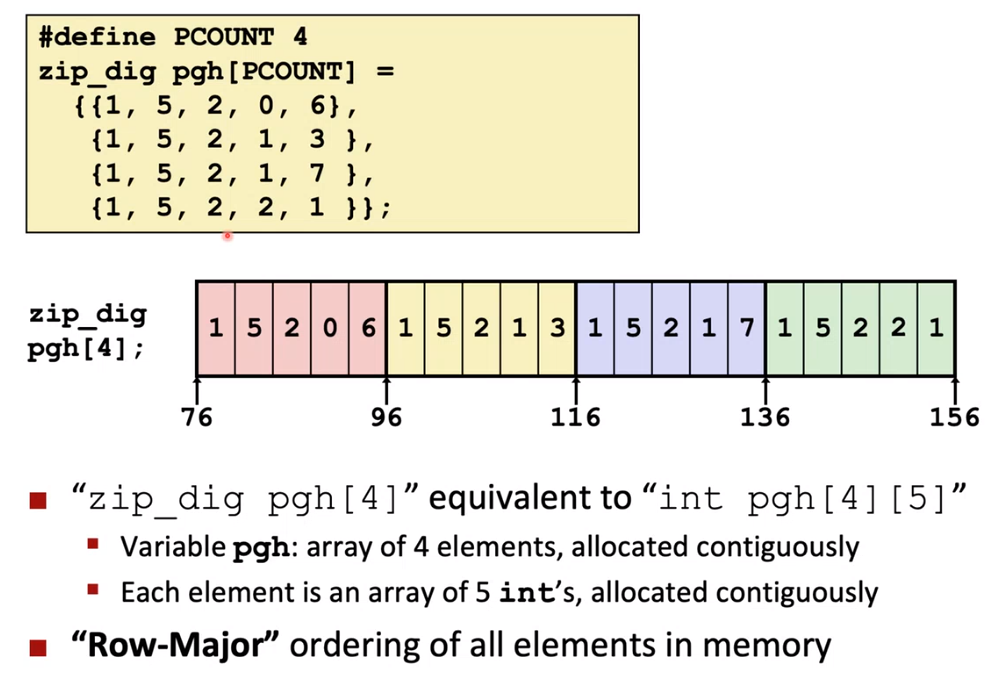
\includegraphics[scale = 0.2]{./figures/nestedArrayEx}
        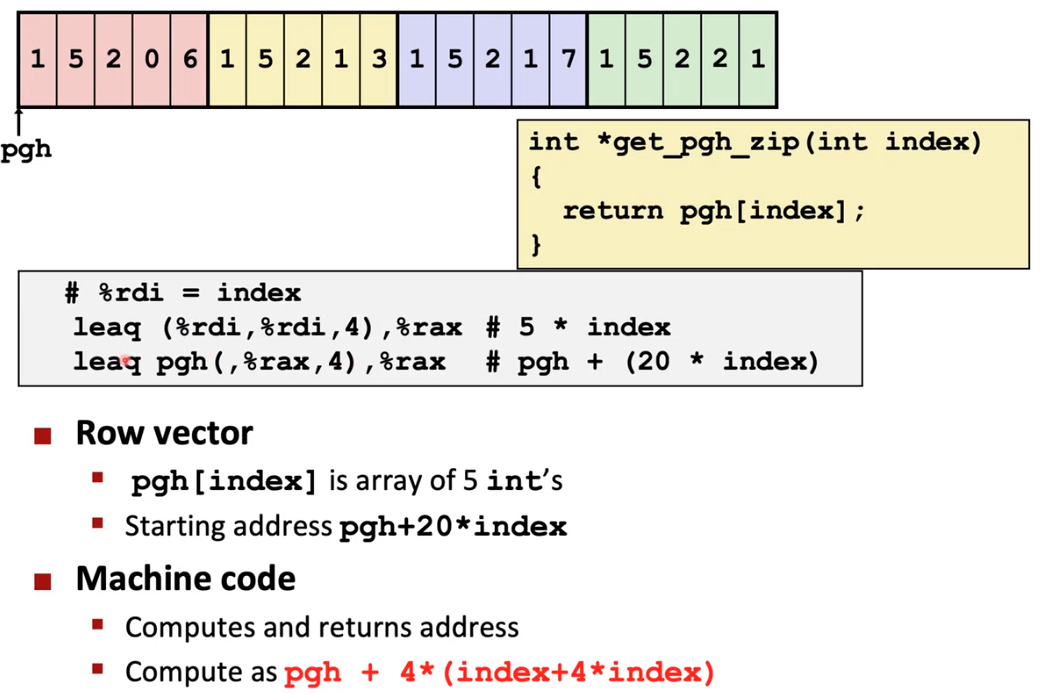
\includegraphics[scale = 0.2]{./figures/nestedArrayEx2}
        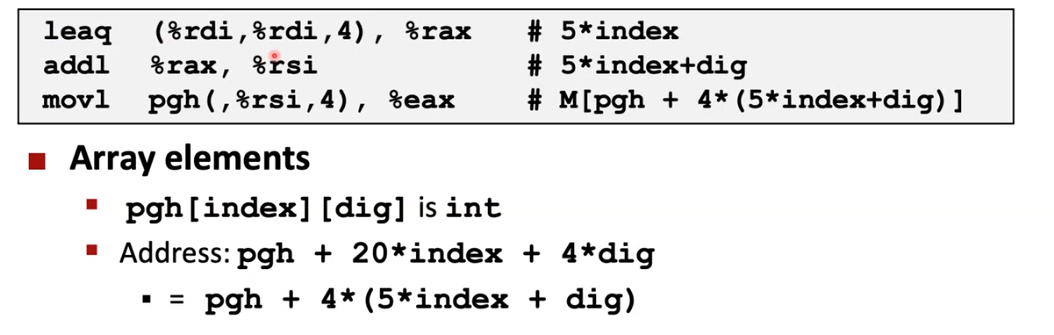
\includegraphics[scale = 0.2]{./figures/nestedArrayEx3}
\end{figure}

We can also make arrays of different structures, for example, the \textbf{Multi-Level Array}:
\begin{figure}[h]
        \centering
        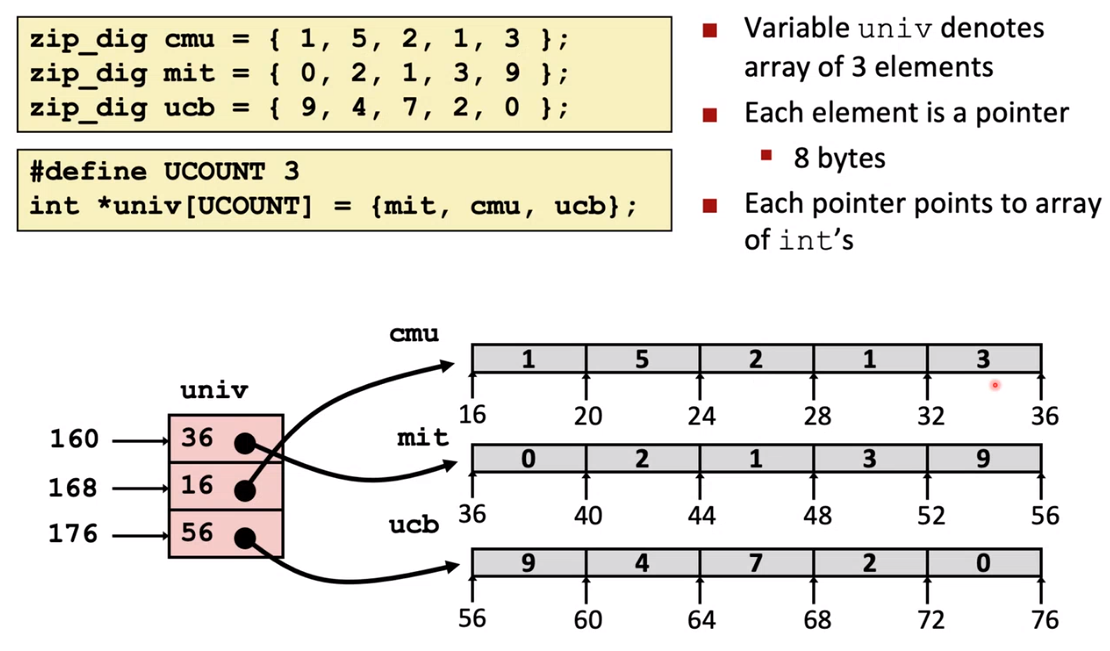
\includegraphics[scale = 0.3]{./figures/multilevel1}
\end{figure}
\pagebreak

To access the elements in this type of array one could use the following procedure:
\begin{figure}[h]
        \centering
        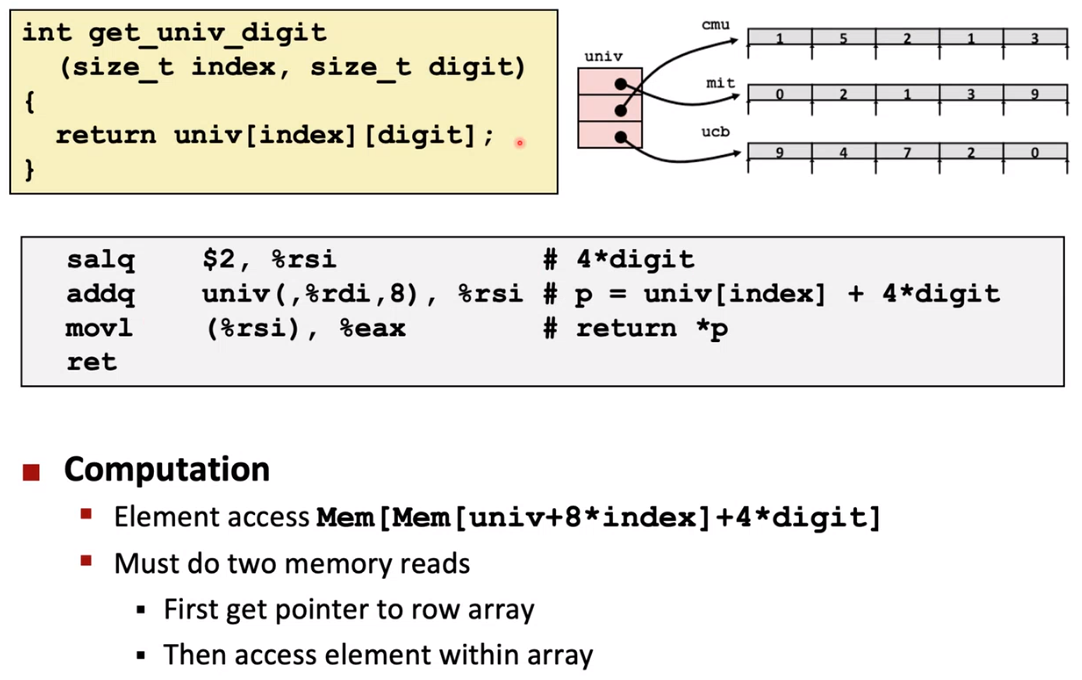
\includegraphics[scale = 0.3]{./figures/multilevel2}
\end{figure}

Note: because this data is not contiguous, the accessing of data may be less efficient.
This can be more clearly seen in the following display:
\begin{figure}[h]
        \centering
        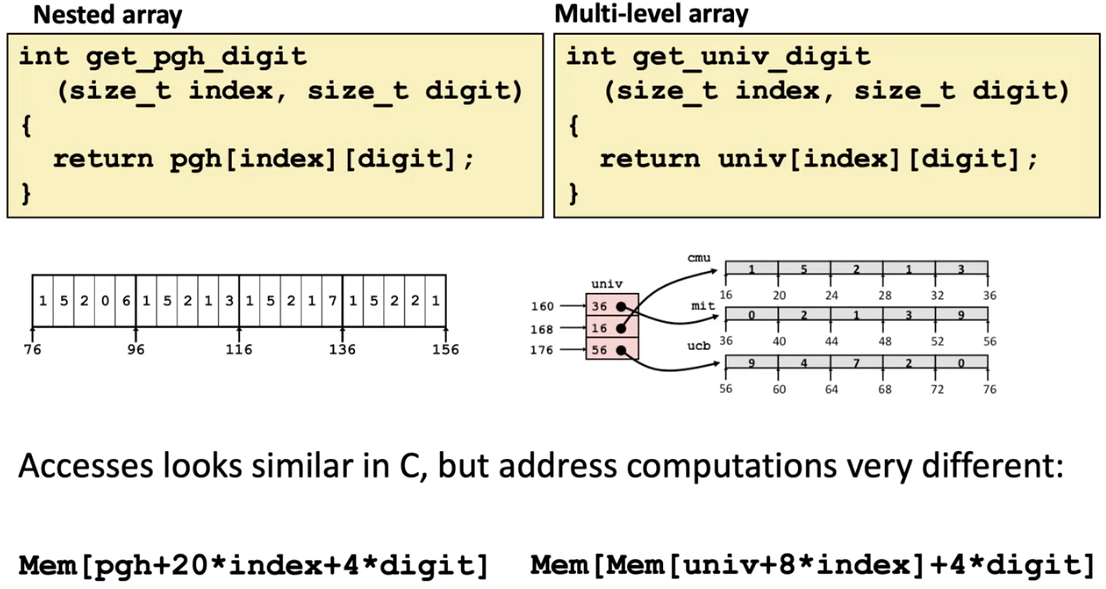
\includegraphics[scale = 0.4]{./figures/arrayVmulti}
\end{figure}
\pagebreak

\subsection*{Code in C}
The representation of an $N\times N$ matrix is C must have fixed dimensions. Indexing the
array can be done either with explicit indexing:
\begin{figure}[h]
        \centering
        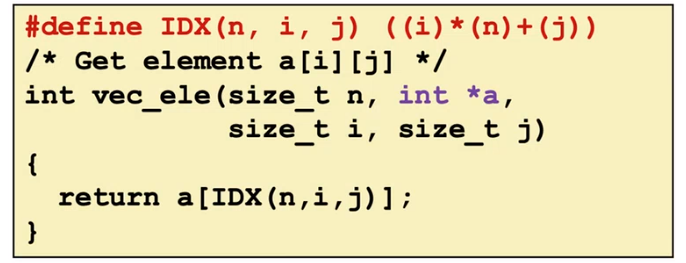
\includegraphics[scale = 0.4]{./figures/indexing1}
\end{figure}

Or by using implicit indexing (Now Supported by gcc!):
\begin{figure}[h]
        \centering
        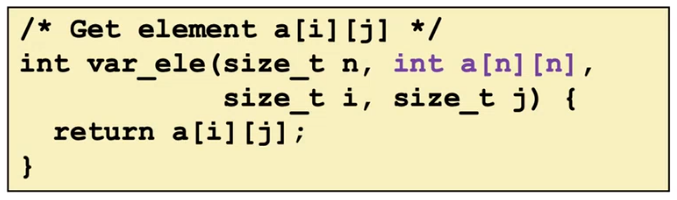
\includegraphics[scale = 0.4]{./figures/indexing2}
\end{figure}

The machine code for this type of access is the following:
\begin{figure}[h]
        \centering
        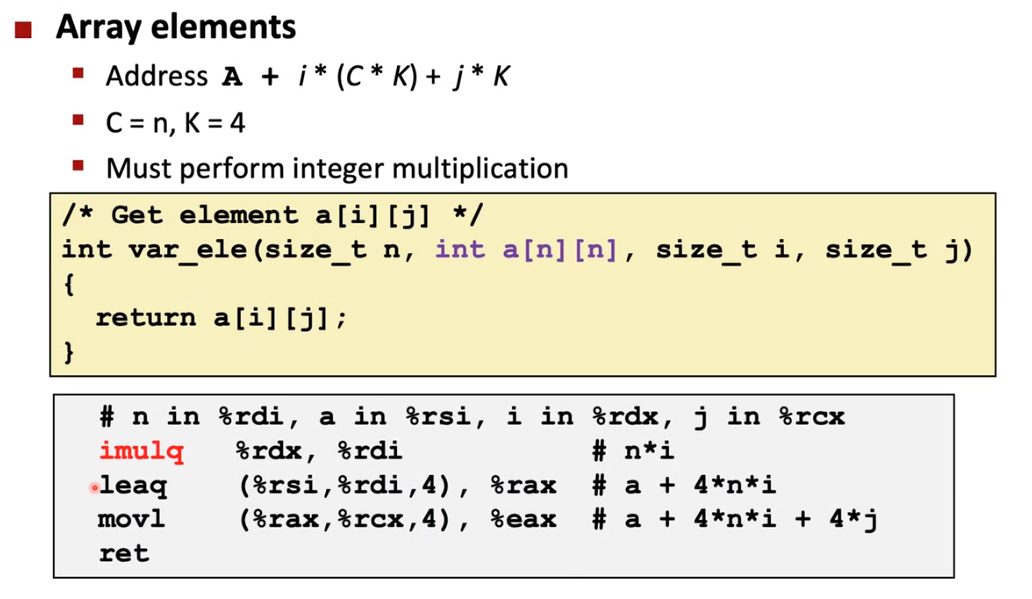
\includegraphics[scale = 0.4]{./figures/nxnindexing}
\end{figure}
\end{document}

